\chapter{Interfaz de Comunicación y Lógica de Control en LabVIEW}
\lineaLateral

\begin{resumenCapitulo}
	En este capítulo se describe el desarrollo de una interfaz de control robusta y versátil, diseñada bajo un esquema de comunicación serial (UART) que permite la compatibilidad con cualquier microcontrolador que soporte este estándar. A continuación, se detalla la implementación de la lógica interna, la estructuración de datos y el protocolo de comunicación desarrollado para garantizar el determinismo en el control del sistema.
\end{resumenCapitulo}

\section{Especificaciones Técnicas del Controlador: ATMega2560}
El núcleo del sistema de control es el microcontrolador de 8 bits \textbf{ATMega2560}, basado en la arquitectura RISC avanzada de Harvard. Esta elección técnica se justifica por su capacidad de procesamiento paralelo de instrucciones en un solo ciclo de reloj, optimizando el \textit{throughput} para tareas de control en tiempo real.

\subsection{Arquitectura y Capacidad de Procesamiento}
El procesador opera a una frecuencia de oscilación de \textbf{16 MHz} mediante un cristal de cuarzo externo. Esto se traduce en una velocidad de ejecución cercana a los \textbf{16 MIPS} (millones de instrucciones por segundo), permitiendo que la mayoría de las instrucciones se completen en un periodo de reloj de tan solo \textbf{62.5 ns}. Esta velocidad es crítica para la gestión del lazo de control de 4 ms y la lectura de los encoders de cuadratura, donde la latencia de respuesta define la estabilidad del brazo.

\subsection{Resolución y Gestión de Señales PWM}
Para el accionamiento de los puentes H (BTS7960) que controlan los motores de corriente continua, el Arduino Mega dispone de 15 canales de modulación por ancho de pulso (PWM) generados por hardware.
\begin{itemize}
	\item \textbf{Resolución Temporal:} Por defecto, el sistema opera con una resolución de \textbf{8 bits} ($2^8 = 256$ niveles de duty cycle), lo que permite un control granular de la velocidad de los motores.
	\item \textbf{Frecuencias de Conmutación:} Las frecuencias de PWM están determinadas por los divisores de frecuencia (\textit{prescalers}) de los temporizadores internos. En la configuración estándar, los pines 4 y 13 operan a aproximadamente \textbf{980 Hz}, mientras que el resto de los pines PWM operan a \textbf{490 Hz}. Esta frecuencia es suficiente para minimizar el rizado de corriente en los devanados del motor sin inducir pérdidas excesivas por conmutación en los MOSFETs del driver.
\end{itemize}


\subsection{Temporización e Interrupciones (Timers)}
La característica más potente del ATMega2560 para este proyecto es su sistema de temporizadores. El microcontrolador integra 6 \textit{timers}: dos de 8 bits y cuatro de \textbf{16 bits} (Timer 1, 3, 4 y 5).
\begin{itemize}
	\item \textbf{Timer 5 (16-bit):} Se utiliza específicamente para generar la base de tiempo determinista del sistema. Al operar con una resolución de 16 bits, permite una configuración extremadamente precisa de interrupciones para el conteo de pasos de los encoders y el envío de telemetría, evitando el \textit{jitter} que ocurriría en un ciclo de \textit{polling} convencional.
	\item \textbf{Vectores de Interrupción:} El controlador soporta hasta 8 interrupciones externas (INT0-INT7) y múltiples interrupciones por cambio de pin (PCINT), permitiendo que los flancos de subida y bajada de los encoders de cuadratura activen rutinas de servicio de interrupción (ISR) de baja latencia.
\end{itemize}

\subsection{Recursos de Memoria y Comunicación}
\begin{itemize}
	\item \textbf{Memoria Flash (256 KB):} Espacio suficiente para almacenar la máquina de estados compleja y las tablas de datos para las rutinas de movimiento.
	\item \textbf{SRAM (8 KB):} Crucial para el manejo de las estructuras (\texttt{Motor\_t}) y los buffers de comunicación serial sin riesgo de desbordamiento de pila.
	\item \textbf{Interfaces UART:} Cuenta con 4 puertos UART independientes, lo que permite mantener la comunicación con LabVIEW a \textbf{500,000 baudios} en el puerto 0, mientras se procesan simultáneamente los datos del Joystick Bluetooth en el puerto 1.
\end{itemize}

\begin{figure}[h]
	\centering
	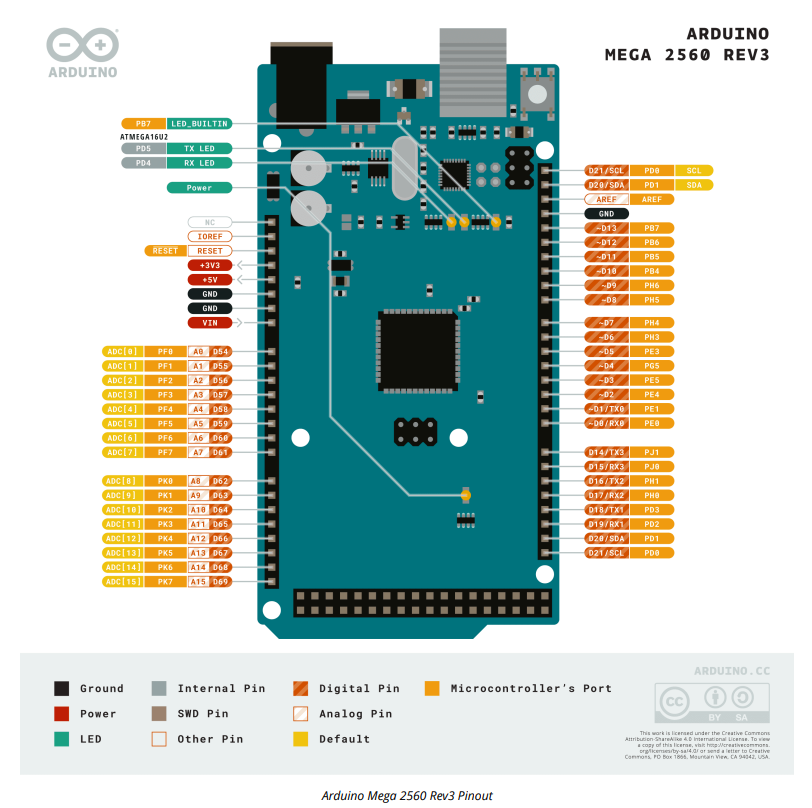
\includegraphics[width=0.7\linewidth]{images/Interfaz/ardMega}
	\caption[Topología.]{Topología del arduino Mega.}
	\label{fig:ardmega}
\end{figure}


\section{Protocolo de Comunicación: Estructura y Fiabilidad}
Inspirado en el estándar industrial Modbus, se implementó un protocolo de comunicación binario personalizado. La elección de un formato binario sobre uno de texto (como strings de comandos) responde a la necesidad de optimizar el ancho de banda y reducir la latencia de procesamiento.



La trama de datos consta de un paquete de \textbf{31 bytes} diseñado para ser decodificado eficientemente en LabVIEW. Esta estructura asegura que no se pierda la integridad del mensaje mediante los siguientes campos:

\begin{itemize}
	\item \textbf{Cabecera (Header):} Un byte de sincronización (0xAA) que indica el inicio de la trama.
	\item \textbf{Estado de Motores:} Un arreglo de 3 bytes donde se empaquetan los estados lógicos de los 6 motores.
	\item \textbf{Finales de Carrera:} Un byte dedicado a reportar el estado de los sensores de límite, permitiendo una reacción inmediata ante colisiones.
	\item \textbf{Telemetría de Pasos:} 24 bytes que contienen la posición actual (int32\_t) de cada uno de los encoders.
	\item \textbf{Ciclo de Redundancia Cíclica (CRC-8):} Un mecanismo de verificación que suma los bytes previos para asegurar que los datos no se corrompieron durante la transmisión.
\end{itemize}

Esta arquitectura es la mejor opción para el proyecto, ya que permite una reestructuración sencilla en LabVIEW mediante el bloque \textit{Unflatten from String}, manteniendo una comunicación confiable y determinista.

\section{Definición del Protocolo de Comunicación}
La comunicación entre LabVIEW y el Arduino Mega se rige por una trama binaria de longitud fija de 31 bytes. A continuación, se presenta el mapa de memoria de la trama enviada desde el controlador:

\begin{table}[h]
	\centering
	\small
	\renewcommand{\arraystretch}{1.5}
	% Usamos tabularx para forzar el ancho total a la línea de texto
	\begin{tabularx}{\textwidth}{|X|X|X|X|X|X|}
		\hline
		\rowcolor{green!20}
		\centering \textbf{Sincronía} & \centering \textbf{ID} & \centering \textbf{Sensores} & \centering \textbf{Estados} & \centering \textbf{Posicionamiento} & \centering \textbf{Verificación} \tabularnewline \hline
		\centering Header & \centering Funct. & \centering Límites & \centering Motores 0-5 & \centering Motor 0 \dots Motor 5 & \centering CRC-8 \tabularnewline \hline
		\centering 1 Byte & \centering 1 Byte & \centering 1 Byte & \centering 3 Bytes & \centering 24 Bytes (4 por eje) & \centering 1 Byte \tabularnewline \hline
	\end{tabularx}
	\caption{Estructura macro de la trama de telemetría.}
\end{table}

\begin{table}[h!]
	\centering
	\small
	\renewcommand{\arraystretch}{1.3} % Un poco más de espacio para que se vea mejor sin bordes verticales
	\caption{Desglose detallado del paquete de datos (31 Bytes).}
	\label{tab:protocolo_detallado}
	% Eliminamos los '|' para quitar los bordes de las columnas
	\begin{tabularx}{\textwidth}{lllX}
		\hline
		\rowcolor{green!20} 
		\textbf{Byte(s)} & \textbf{Campo} & \textbf{Tipo de Dato} & \textbf{Descripción Técnica} \\ \hline
		0 & Header & \texttt{uint8\_t} & Byte de sincronía constante (\texttt{0xAA}). \\ \hline
		1 & Función & \texttt{uint8\_t} & Identificador del modo de operación activo. \\ \hline
		2 & Límites & \texttt{uint8\_t} & Estado de finales de carrera (Lógica NC). \\ \hline
		3 -- 5 & Edo. Motores & \texttt{uint8\_t[3]} & Bit-packing de estados (3 bits/motor). \\ \hline
		6 -- 9 & Pasos M0 & \texttt{int32\_t} & Posición actual Eje 1 (Base). \\ \hline
		10 -- 13 & Pasos M1 & \texttt{int32\_t} & Posición actual Eje 2 (Hombro). \\ \hline
		14 -- 17 & Pasos M2 & \texttt{int32\_t} & Posición actual Eje 3 (Codo). \\ \hline
		18 -- 21 & Pasos M3 & \texttt{int32\_t} & Posición actual Eje 4 (Pitch). \\ \hline
		22 -- 25 & Pasos M4 & \texttt{int32\_t} & Posición actual Eje 5 (Roll). \\ \hline
		26 -- 29 & Pasos M5 & \texttt{int32\_t} & Posición actual Eje 6 (Gripper/Giro). \\ \hline
		30 & CRC & \texttt{uint8\_t} & Checksum de integridad (Suma de bytes). \\ \hline
	\end{tabularx}
\end{table}
\section{Implementación de Estructuras de Datos en C}
Para optimizar el firmware, se implementaron estructuras (\texttt{struct}) que permiten un manejo eficiente de la memoria y facilitan el mantenimiento del código. En el contexto de un microcontrolador de 8 bits, esta organización es fundamental para el manejo de múltiples periféricos de forma concurrente.

En este proyecto destacan dos estructuras principales:
\begin{enumerate}
	\item \textbf{\texttt{Motor\_t}:} Encapsula los parámetros operativos de cada articulación, incluyendo pines de PWM, contadores de encoders, variables de error y estados de reporte. Esto permite una abstracción donde cada eje se gestiona como una entidad independiente.
	\item \textbf{\texttt{MsgDatos\_t}:} Estructura diseñada bajo el concepto de empaquetamiento de memoria, que representa fielmente la trama de 31 bytes. Esto asegura que la disposición de los datos en la SRAM coincida exactamente con la secuencia de transmisión UART.
\end{enumerate}

\section{Implementación de Estructuras de Datos en C}
Para el desarrollo del firmware, se utilizaron estructuras (\texttt{struct}) en lenguaje C. El uso de estas permite encapsular variables relacionadas bajo un mismo nombre, facilitando la organización del código y el paso de datos entre funciones de control y comunicación.

\begin{lstlisting}[language=C++, caption={Estructura de control para articulaciones individuales}, label={lst:motor_struct}]
	typedef struct {
		uint8_t pinPWM;       // Pin de control de velocidad
		uint8_t pinDir;       // Pin de sentido de giro
		int32_t pasosActuales; // Contador de pasos (encoder)
		int32_t pasosMeta;     // Objetivo de posicionamiento
		uint8_t estadoModo;    // Modo activo (IDLE, FAST, FOLLOW)
		bool limiteActivado;   // Flag de seguridad (NC)
	} Motor_t;
\end{lstlisting}

La segunda estructura fundamental es la que define el paquete de telemetría. Al utilizar el atributo \texttt{packed}, aseguramos que no existan espacios de relleno (\textit{padding}) entre los miembros de la estructura, garantizando que el tamaño total sea de exactamente 31 bytes para coincidir con la trama de LabVIEW.

\begin{lstlisting}[language=C++, caption={Estructura de la trama de telemetría (31 Bytes)}, label={lst:msgdatos_struct}]
	typedef struct __attribute__((packed)) {
		uint8_t header;         // Byte de sincronia (0xAA)
		uint8_t idFuncion;      // Identificador de comando
		uint8_t limites;        // Bits de sensores de carrera
		uint8_t estados[3];     // Estados de los 6 motores
		int32_t posiciones[6];  // Encoders de 32 bits por eje
		uint8_t crc;            // Checksum de verificacion
	} MsgDatos_t;
\end{lstlisting}

\section{Definición de Enumeraciones (Enums)}
Para garantizar la integridad de la máquina de estados y optimizar la comunicación serial, se implementaron enumeraciones que separan la lógica de control interno de los reportes enviados a la interfaz de usuario.

\begin{lstlisting}[language=C++, caption={Enumeradores para reportes y comportamientos del sistema}, label={lst:enums_sistema}]
	// Reporta a Labview el estado simplificado (Maximo 8 estados)
	enum EstadoReporte {
		LV_IDLE = 0,          // 000: Quieto / Esperando
		LV_MOVIENDO = 1,      // 001: Ejecutando trayectoria o comando manual
		LV_HOMING = 2,        // 010: En proceso de busqueda de cero
		LV_ERROR_TRABADO = 3  // 011: Meta no alcanzada / Obstruccion
	};
	
	// Define el modo de operacion solicitado por el controlador
	enum Comportamiento_t {
		MODE_IDLE = 0,           // Reposo activo
		MODE_FAST_MOV = 1,       // Movimiento rapido (Jogging)
		MODE_MOVE_DEG = 2,       // Posicionamiento por grados
		MODE_FOLLOW_ROUTINE = 3, // Ejecucion de trayectorias (Excel)
		MODE_HOMING = 4,         // Rutina de referenciado
		MODE_EMERGENCY_STOP = 5  // Paro de emergencia inmediato
	};
\end{lstlisting}

Adicionalmente, se utiliza un enumerador específico para la gestión detallada de la lógica de control interna. Este permite que cada articulación rastree su progreso durante tareas complejas como el referenciado (\textit{Homing}) o el posicionamiento punto a punto.

\begin{lstlisting}[language=C++, caption={Enumeradores para la logica interna de control}, label={lst:enums_internos}]
	// Mantiene la logica completa para el control de pasos interno
	enum MaqEstado_t {
		MQ_IDLE = 1,      // Motor en espera
		MQ_HOMING = 2,    // Ejecutando fase de busqueda
		MQ_MOVIENDO = 3,  // En transito hacia la meta
		MQ_META = 4       // Posicion alcanzada con exito
	};
	
	// Fases individuales para la rutina de referenciado
	enum Homing_t {
		MAQ_HOMING_F1 = 1, // Busqueda rapida de sensor
		MAQ_HOMING_F2 = 2, // Retroceso de precision
		MAQ_HOMING_F3 = 3  // Ajuste final de cero
	};
\end{lstlisting}

Esta distinción es fundamental para el determinismo del sistema. Mientras que la lógica interna utiliza estados detallados para el control de los motores, la telemetría enviada a LabVIEW se compacta en el enumerador \texttt{EstadoReporte} para cumplir con la restricción de 3 bits por motor dentro de la trama de 31 bytes.

\section{Restricciones de Hardware y Determinismo}
La arquitectura basada en el ATMega2560 requiere una gestión estricta de los tiempos de ciclo. El proceso de envío serial, al ser asíncrono y dependiente de un buffer, puede comprometer la estabilidad del sistema si no se regula adecuadamente. 

Se estableció un \textbf{periodo de control determinista de 4ms (250 Hz)}. La prioridad del procesador se asignó a la actualización de encoders mediante interrupciones y a la lógica de control de los puentes H. El envío de telemetría está sincronizado para ejecutarse al final de cada ciclo, garantizando que el sistema mantenga un tiempo de respuesta constante y predecible bajo cualquier condición de carga.

\section{Máquina de Estados de Control de Movimiento}
La lógica de operación reside en la función \texttt{actualizarLogicaMotor}, una máquina de estados finitos (FSM) que gobierna el comportamiento dinámico del brazo Mitsubishi. La transición entre estados depende tanto de los comandos recibidos vía LabVIEW como de las condiciones de seguridad detectadas por hardware.

Los estados operativos definidos son:
\begin{itemize}
	\item \textbf{MODE\_IDLE:} Estado de seguridad predeterminado. Los motores se mantienen en frenado activo para contrarrestar el torque inducido por la gravedad en las articulaciones.
	\item \textbf{MODE\_FAST\_MOV:} Modo de desplazamiento rápido orientado a operaciones de posicionamiento manual (\textit{Jogging}). Permite movimientos precisos basados en los deltas de pasos enviados desde la interfaz.
	\item \textbf{MODE\_FOLLOW\_ROUTINE:} Modo de ejecución de trayectorias. El sistema procesa vectores de PWM y tiempos de ejecución provenientes de archivos de datos, utilizando temporizadores internos para asegurar la detención precisa del movimiento.
\end{itemize}



\begin{center}
	\small
	\renewcommand{\arraystretch}{1.2}
	\begin{tabular}{c}
		\fcolorbox{green!30!black}{green!5}{\textbf{Lectura Serial UART}} \\
		$\downarrow$ \\
		\fcolorbox{green!30!black}{white}{\textbf{¿CRC Válido?}} $\xrightarrow{\text{No}}$ \fbox{Ignorar Paquete} \\
		$\downarrow$ \scriptsize{Sí} \\
		\fcolorbox{green!30!black}{white}{\textbf{¿Choque (Límites)?}} $\xrightarrow{\text{Sí}}$ \fbox{MODE\_IDLE (Freno)} \\
		$\downarrow$ \scriptsize{No} \\
		\fcolorbox{green!30!black}{green!5}{\textbf{Ejecutar Modo (FAST / FOLLOW / JOY)}}
	\end{tabular}
\end{center}

\section{Adquisición de Datos y Gestión de Periféricos I/O}
La interacción con el brazo Mitsubishi Move Master EX requiere la gestión precisa de tres tipos de señales críticas: la retroalimentación de posición (encoders), la detección de límites físicos (finales de carrera) y el control de estabilidad (frenos electromecánicos).

\subsection{Retroalimentación de Posición vía Encoders}
A diferencia de los sistemas basados en interrupciones externas que pueden saturar el procesador a altas velocidades, se implementó una estrategia de \textbf{muestreo periódico}. Los estados de las fases A y B de cada encoder son leídos cada cierto tiempo dentro de una interrupción de temporizador (\textit{Timer Interrupt}). 

Esta técnica permite filtrar el ruido electrónico y asegura que el conteo de pasos sea determinista, evitando que el microcontrolador pierda ciclos de ejecución críticos para la comunicación serial. Los valores acumulados se almacenan en variables de tipo \texttt{int32\_t} dentro de la estructura \texttt{Motor\_t} para su posterior envío a LabVIEW.

\subsection{Detección de Límites (Finales de Carrera)}
El robot cuenta con interruptores de límite en configuración Siempre Abierta (NO). Para mejorar la experiencia de usuario y la interpretación de datos en la interfaz de LabVIEW, se implementó una inversión lógica en el firmware. 

Aunque el hardware detecta una transición física, el código procesa esta señal para \textbf{retornar un valor booleano TRUE} únicamente cuando el sensor está siendo presionado. Esta abstracción facilita la lógica de seguridad en la interfaz, permitiendo que el operario identifique visualmente el estado de colisión o límite de manera intuitiva y directa.

\subsection{Control de Frenos Electromecánicos}
Los frenos del robot son dispositivos de seguridad que evitan el colapso de las articulaciones por gravedad cuando los motores no están energizados. Su estado se gestiona mediante lecturas digitales directas (\texttt{digitalRead}), las cuales son integradas en la trama de telemetría. Esta adquisición permite que LabVIEW confirme en tiempo real si el brazo se encuentra en estado de liberación para movimiento o bajo retención de seguridad.

\begin{lstlisting}[language=C++, caption={Lógica de lectura de señales digitales y acondicionamiento}, label={lst:lectura_sensores}]
	// Lectura de finales de carrera con logica positiva para la interfaz
	uint8_t leerFinalesCarrera() {
		uint8_t estadoByte = 0;
		for (int i = 0; i < NUM_FINAL_C; i++) {
			// Se retorna TRUE si el sensor esta presionado
			if (digitalRead(PIN_FINAL_CARRERA[i]) == HIGH) {
				estadoByte |= (1 << i);
			}
		}
		return estadoByte;
	}
	
	// Monitoreo de estado de frenos
	void monitorearFrenos() {
		bool estadoFreno1 = digitalRead(PIN_FRENO[0]);
		bool estadoFreno2 = digitalRead(PIN_FRENO[1]);
		// Logica de seguridad integrada...
	}
\end{lstlisting}

\subsection{Procesamiento de Encoders y Optimización por Hardware}

Para la lectura de los encoders, se descartó el uso de interrupciones externas convencionales (\textit{External Interrupts}), ya que la alta frecuencia de pulsos generada por los cinco motores simultáneamente saturaba el procesador, provocando un comportamiento errático en el giro de los motores y pérdida de pasos. 

En su lugar, se implementó una estrategia de \textbf{muestreo por interrupción de temporizador (Timer Interrupt Handling)} utilizando el Timer 5 del ATMega2560.

\subsubsection{Configuración del Timer 5 y Resolución de Pasos}
El Timer 5 se configuró en modo CTC (\textit{Clear Timer on Compare Match}) con un valor de comparación de 199 y un prescaler de 8. Esto genera una frecuencia de muestreo de 10 kHz (cada 100 $\mu$s). Esta frecuencia es lo suficientemente alta para capturar todos los cambios de fase sin sobrecargar la CPU, permitiendo que el hilo principal del programa ejecute la lógica de control y comunicación sin retardos.

En cuanto a la resolución, se implementó una decodificación de tipo \textbf{Half-Quad}. Aunque el disco físico del encoder del Mitsubishi Move Master EX posee 200 ranuras, la lógica de software permite detectar cambios de estado específicos que duplican la resolución efectiva a 400 pasos por revolución, logrando un equilibrio ideal entre precisión posicional y carga computacional.

\subsubsection{Algoritmo de Tabla de Búsqueda (Look-up Table)}
Para determinar el sentido de giro y el conteo de pasos de forma ultra rápida dentro de la ISR (\textit{Interrupt Service Routine}), se utilizó una tabla de estados precalculada:

\begin{lstlisting}[language=C++, caption={Tabla de estados para decodificacion de Encoders}, label={lst:encoder_table}]
	const int8_t encoderTable[16] = {
		0, 0, 0, 0,   // Sin cambio o estados invalidos
		1, 0, 0, -1,  // Incremento detectado / Error
		-1, 0, 0, 1,   // Decremento detectado / Error
		0, 0, 0, 0    // Sin cambio o estados invalidos
	};
\end{lstlisting}

La lógica consiste en concatenar el estado anterior de las fases A y B con el estado actual, formando un índice de 4 bits (valores de 0 a 15). Este índice accede directamente a la tabla, la cual devuelve un \textbf{1} para incrementar, un \textbf{-1} para decrementar o un \textbf{0} si no hubo cambio o si el cambio detectado es físicamente imposible (ruido).

\subsubsection{Pseudocódigo de la Lógica de Lectura}
El siguiente pseudocódigo ilustra la operación realizada cada 100 microsegundos:

\begin{center}
	\begin{minipage}{0.85\textwidth}
		\begin{tcolorbox}[
			colback=green!20,      % Fondo verde pastel
			colframe=green!20,     % Borde del mismo verde pastel
			coltitle=black,        % Titulo en negro
			colupper=black,        % Texto superior en negro
			title=Algoritmo de Muestreo (ISR Timer 5), 
			fonttitle=\bfseries,
			arc=2mm                % Bordes ligeramente redondeados para suavizar la estética
			]
			\small
			\begin{enumerate}
				\item \textbf{Para cada} motor $i$ del 0 al 4:
				\begin{enumerate}
					\item Leer estados físicos de los pines Fase A y Fase B.
					\item Combinar estados: $Actual = (FaseA \ll 1) \text{ OR } FaseB$.
					\item Crear índice: $Indice = (Anterior[i] \ll 2) \text{ OR } Actual$.
					\item Consultar tabla: $Delta = encoderTable[Indice]$.
					\item Actualizar posición: $Pasos[i] = Pasos[i] + Delta$.
					\item Guardar estado para el siguiente ciclo: $Anterior[i] = Actual$.
				\end{enumerate}
				\item \textbf{Fin del ciclo}
			\end{enumerate}
		\end{tcolorbox}
	\end{minipage}
\end{center}

\section{Interfaz de Usuario en LabVIEW}
La estación de control fue desarrollada en LabVIEW, aprovechando su capacidad para la gestión de datos mediante una arquitectura de manejador de mensajes encolados (QMH). La interfaz se organiza en un panel principal con una barra de navegación lateral que permite conmutar entre tres pestañas operativas: \textbf{Dashboard}, \textbf{Control Manual} y \textbf{Control PID}.

\subsection{Panel de Monitoreo (Dashboard)}
La pestaña de \textit{Dashboard} funciona como el centro de diagnóstico principal. En esta vista se presentan indicadores visuales de tipo carátula para cada una de las articulaciones (Cadera, Hombro, Codo, Antebrazo y Muñeca). Para cada eje, el sistema despliega en tiempo real:
\begin{itemize}
	\item \textbf{Conteo de Pasos:} Valor absoluto del encoder tras el procesamiento en el microcontrolador.
	\item \textbf{Velocidad:} Cálculo derivado de la variación de pasos por unidad de tiempo.
	\item \textbf{Estado de Alarmas:} Indicadores de seguridad para los finales de carrera y estados de error.
\end{itemize}

\begin{figure}[h]
	\centering
	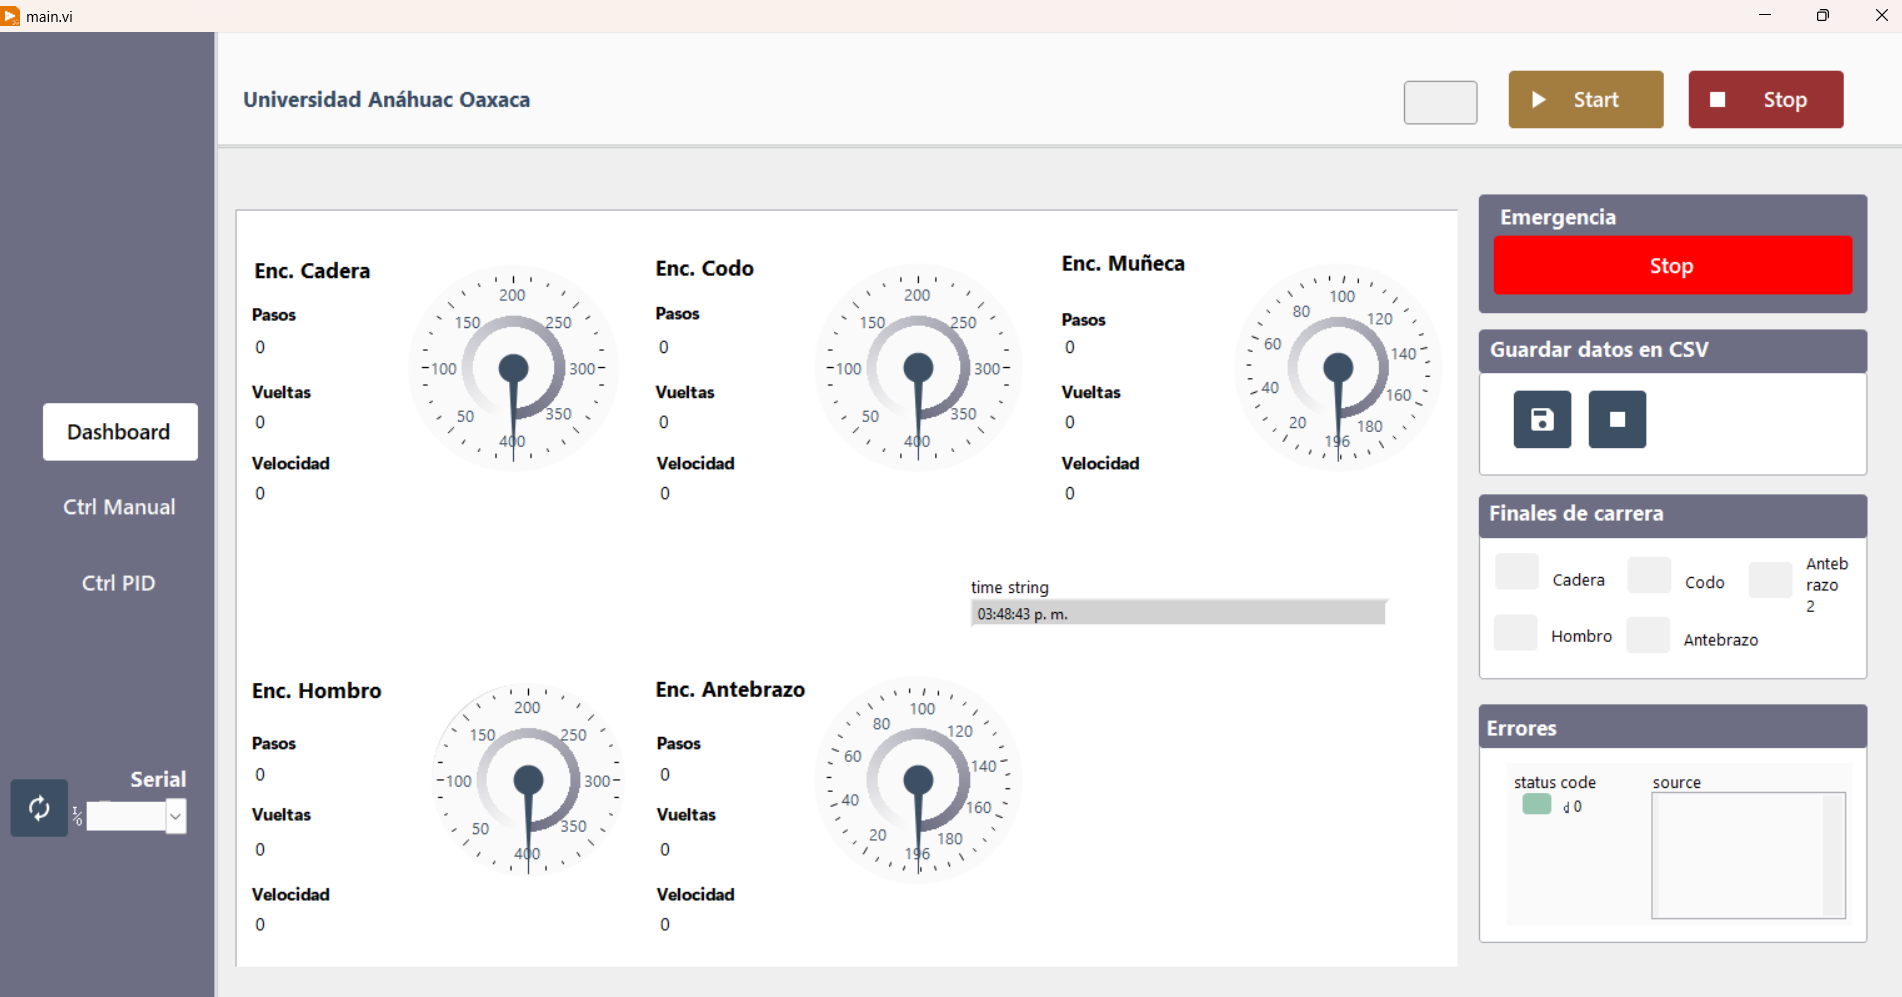
\includegraphics[width=0.5\linewidth]{images/Interfaz/dashboard}
	\caption[Dashboard.]{Ventana de lectura de los encoders.}
	\label{fig:dashboard}
\end{figure}


\subsection{Modos de Control: Manual y Trayectorias}
La pestaña de \textbf{Control Manual} ofrece al operario dos métodos para manipular el brazo:
\begin{enumerate}
	\item \textbf{Control por PWM:} Ajuste directo del ciclo de trabajo para cada motor mediante controles deslizantes (\textit{sliders}), permitiendo movimientos finos para el posicionamiento inicial del robot.
	\item \textbf{Rutina desde Archivo:} Funcionalidad avanzada que permite cargar un archivo externo (CSV o Excel) con trayectorias predefinidas. El sistema lee estas coordenadas y las envía de forma secuencial al controlador para su ejecución automática.
\end{enumerate}

\begin{figure}[h]
	\centering
	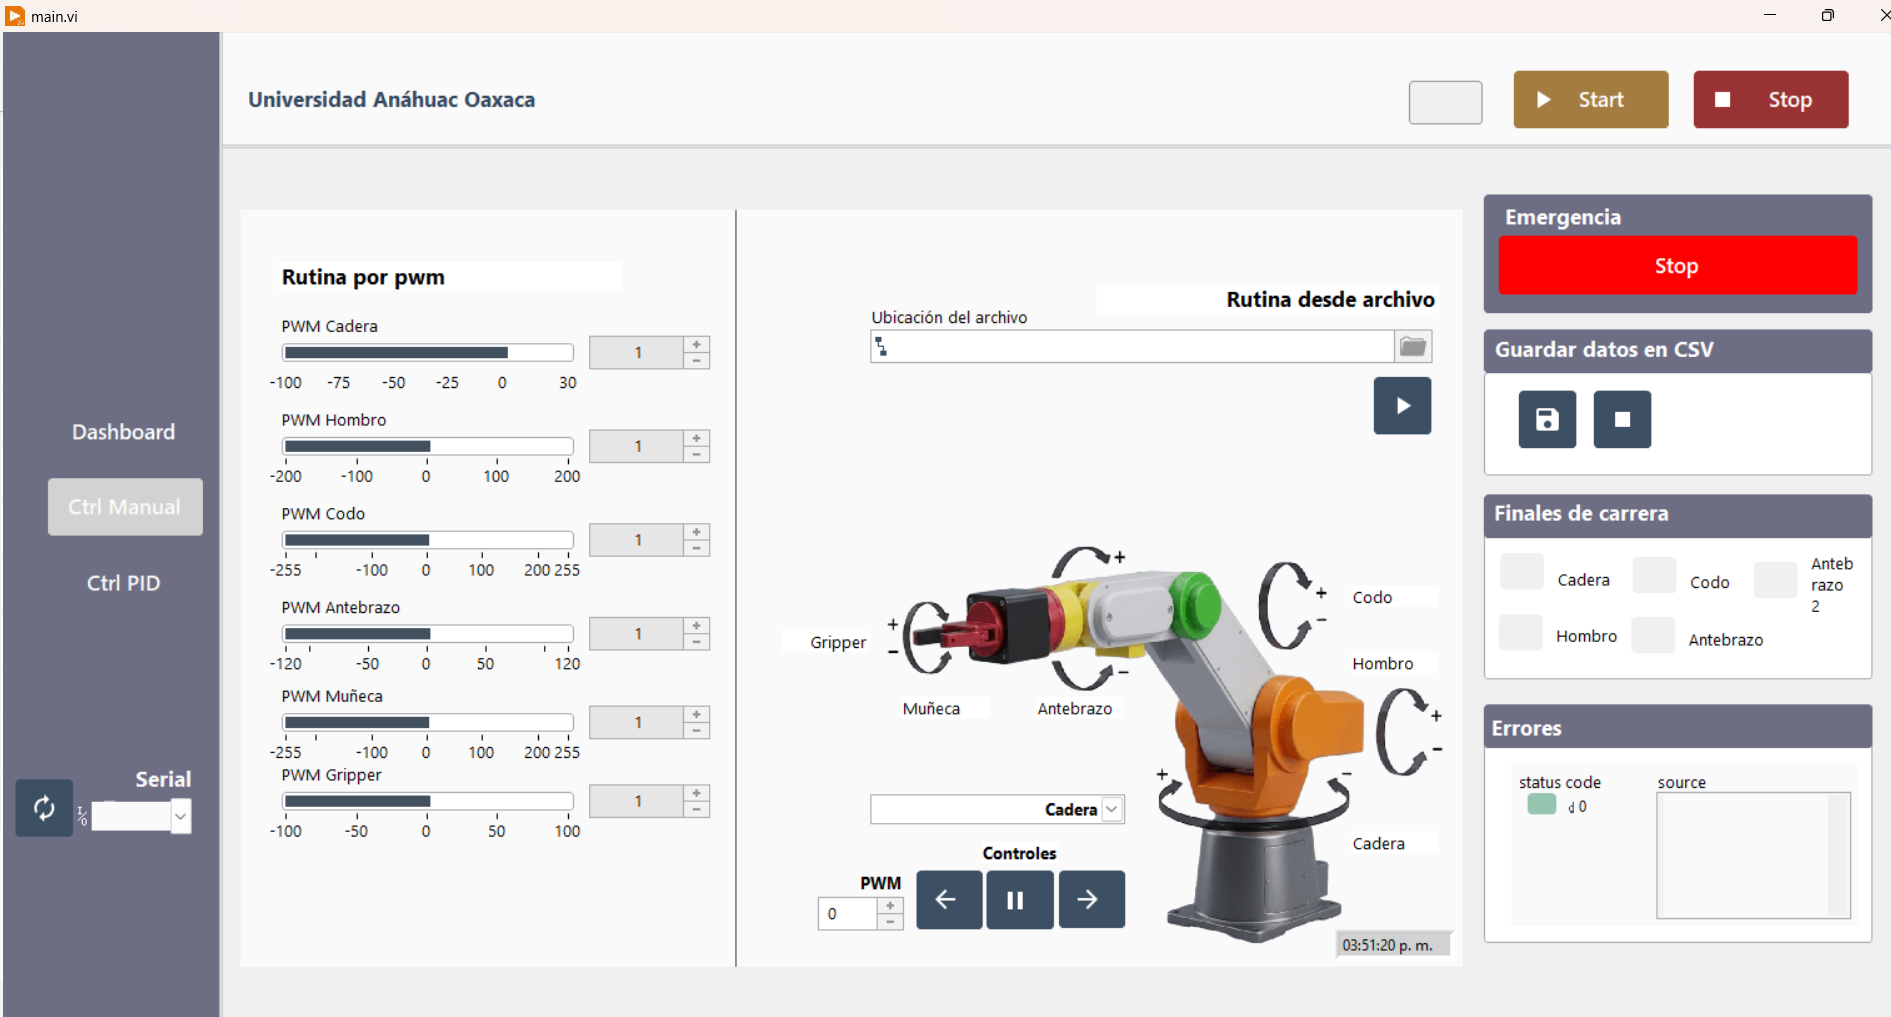
\includegraphics[width=0.7\linewidth]{images/Interfaz/control}
	\caption{Ventana de control de la interfaz.}
	\label{fig:control}
\end{figure}



\subsection{Sintonización y Control PID}
La pestaña de \textbf{Control PID} está diseñada para la optimización dinámica del movimiento. Esta sección permite al usuario ajustar las constantes de control ($K_p$, $T_i$, $T_d$) de manera individual para cada articulación. Incluye una gráfica de tiempo real (\textit{Waveform Chart}) que superpone el \textbf{Setpoint} (posición deseada) frente a la \textbf{Posición Actual}, permitiendo visualizar el error, el sobreimpulso y el tiempo de asentamiento del sistema bajo diferentes condiciones de carga.

\begin{center}
	\fcolorbox{green!30!black}{green!5}{
		\begin{minipage}{0.9\textwidth}
			\textbf{Nota de Seguridad:} Independientemente de la pestaña activa, la interfaz mantiene un botón de \textbf{Paro de Emergencia} global que, al activarse, envía una señal prioritaria para frenar todos los motores y bloquear las articulaciones.
		\end{minipage}
	}
\end{center}

\begin{figure}[h]
	\centering
	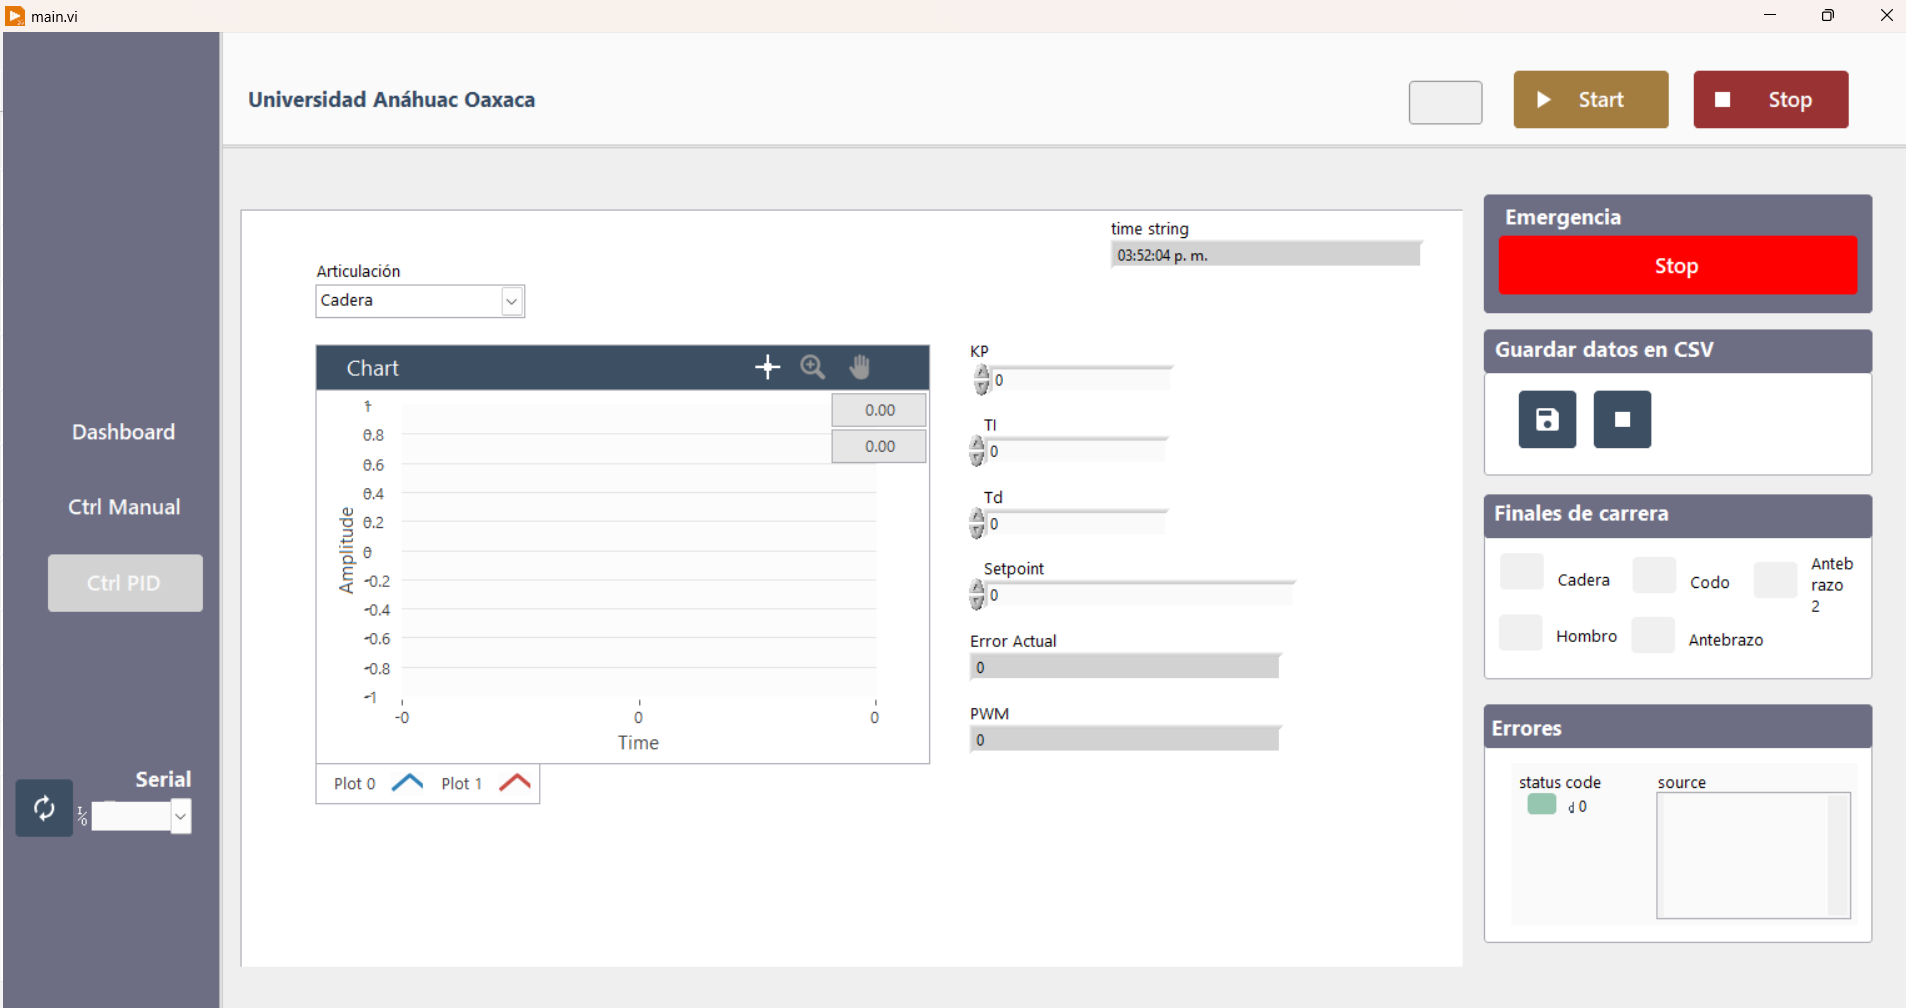
\includegraphics[width=0.7\linewidth]{images/Interfaz/pid}
	\caption{Ventana de PID de la interfaz.}
	\label{fig:pid}
\end{figure}


\begin{resultadosFase}
	\begin{itemize}
		\item \textbf{Comunicación:} Tasa de transferencia de 500,000 baudios con pérdida de datos nula.
		\item \textbf{Precisión:} Ciclo de control estable a 4ms para la actualización de lazo abierto y cerrado.
		\item \textbf{Seguridad:} Respuesta de detención inmediata ante señales de finales de carrera integrada en la máquina de estados.
	\end{itemize}
\end{resultadosFase}